
%(BEGIN_QUESTION)
% Copyright 2006, Tony R. Kuphaldt, released under the Creative Commons Attribution License (v 1.0)
% This means you may do almost anything with this work of mine, so long as you give me proper credit

Fisher modell 846 I/P bruker en interessant strøm-til-trykk-transduserdesign, ment for å levere variabelt lufttrykksignal til posisjoneringsventiler. Et forenklet diagram av mekanismen er vist her:

$$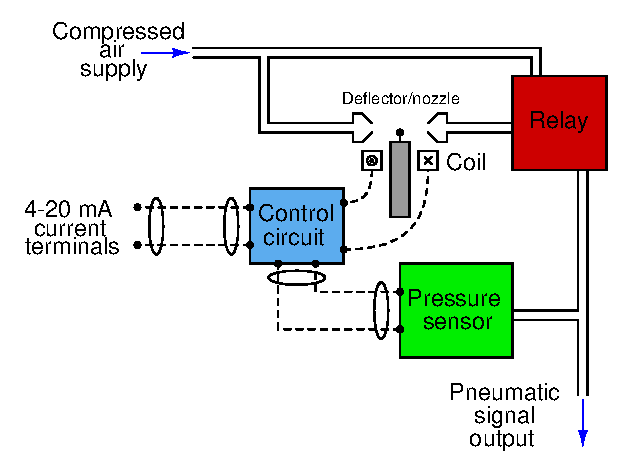
\includegraphics[width=15.5cm]{i00916x01.eps}$$

Forklar hvordan tilbakekoblingssystemet virker i denne designen, og hvordan det skiller seg vesentlig fra klassiske pneumatiske kraftbalanse-I/P-transdusere.

\underbar{file i00916}
%(END_QUESTION)





%(BEGIN_ANSWER)

Tilbakekoblingssløyfen i denne I/P-designen er elektronisk, ikke mekanisk.

%(END_ANSWER)





%(BEGIN_NOTES)

En innebygd fordel med elektronisk tilbakekobling er at den (potensielt) er mer lineær enn mekanisk tilbakekobling. Det er også verdt å merke seg at reléet ligger inne i tilbakekoblingssløyfen. Det betyr at negativ tilbakekobling automatisk vil kompensere for eventuelle iboende ikke-lineariter i reléet. Sammenlign dette med Fisher modell 546 I/P, der det pneumatiske reléet ikke er en del av tilbakekoblingssløyfen, og der total nøyaktighet er svært avhengig av reléets ytelse.

%INDEX% Relay, I/P transducer: Fisher model 846

%(END_NOTES)

